%standard 2.1


%start_of_questions

%new_question
%%%%%%%%%%%%%%%%%%%%%
	% Problem 1
	% Difficulty: 1
%%%%%%%%%%%%%%%%%%%%%
	\item
		%https://edabit.com/challenge/QzXtDnSZL6y4ZcEvT
		A farmer is asking you to tell him how many legs can be counted among all his animals. 
		The farmer breeds three species:
		\begin{itemize}
			\item chickens, which have \textbf{2} legs
			\item cows, which have \textbf{4} legs
			\item pigs, which have \textbf{4} legs
		\end{itemize}
		Write a program that asks the farmer how many of each animal he has, and then outputs the
		total number of legs.  		
		For example, \\ \ \hfill
		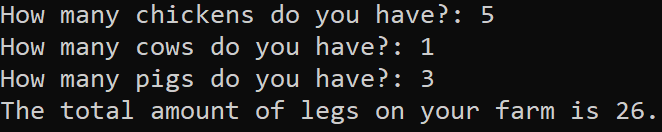
\includegraphics[height = 0.6in]{./imgs/animalLegs_ex1.PNG} \hfill
		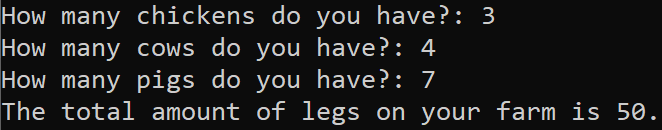
\includegraphics[height = 0.6in]{./imgs/animalLegs_ex2.PNG} \hfill \


%new_question
%%%%%%%%%%%%%%%%%%%%%
	% Problem 2
	% Difficulty: 1
%%%%%%%%%%%%%%%%%%%%%
	\item 
		You are counting points for a basketball game. Ask the user the amount of 3-pointers scored 
		and the amount 2-pointers scored, find the final points for the team and output the value.\\
		For example, if a team scored 5 2-pointers and 7 3-pointers, then their score would be 31.\\
		If a team scored 6 2-pointers and 5 3-pointers, then their score would be 27.

%end_of_questions


